\section{应用成效}\label{sec:results}
\subsection{成果展示}
\subsubsection{功能实现情况}
系统已完整实现表\ref{tab:requirements}中的全部功能需求：选择地区与日期即可回放任一测试日的次日需水预测、90\%预测区间、昨日值基线和事后参考值；输入土壤与设备参数后实时给出是否灌溉、毛灌溉量、净补水量和补水后预计亏缺；供水不足时自动提示；每次结果可导出为JSON决策记录。“模型验证”与“策略回测”视图集中展示本章的主要实验结果（图\ref{fig:evidence-ui}）。

\begin{figure}[H]\centering
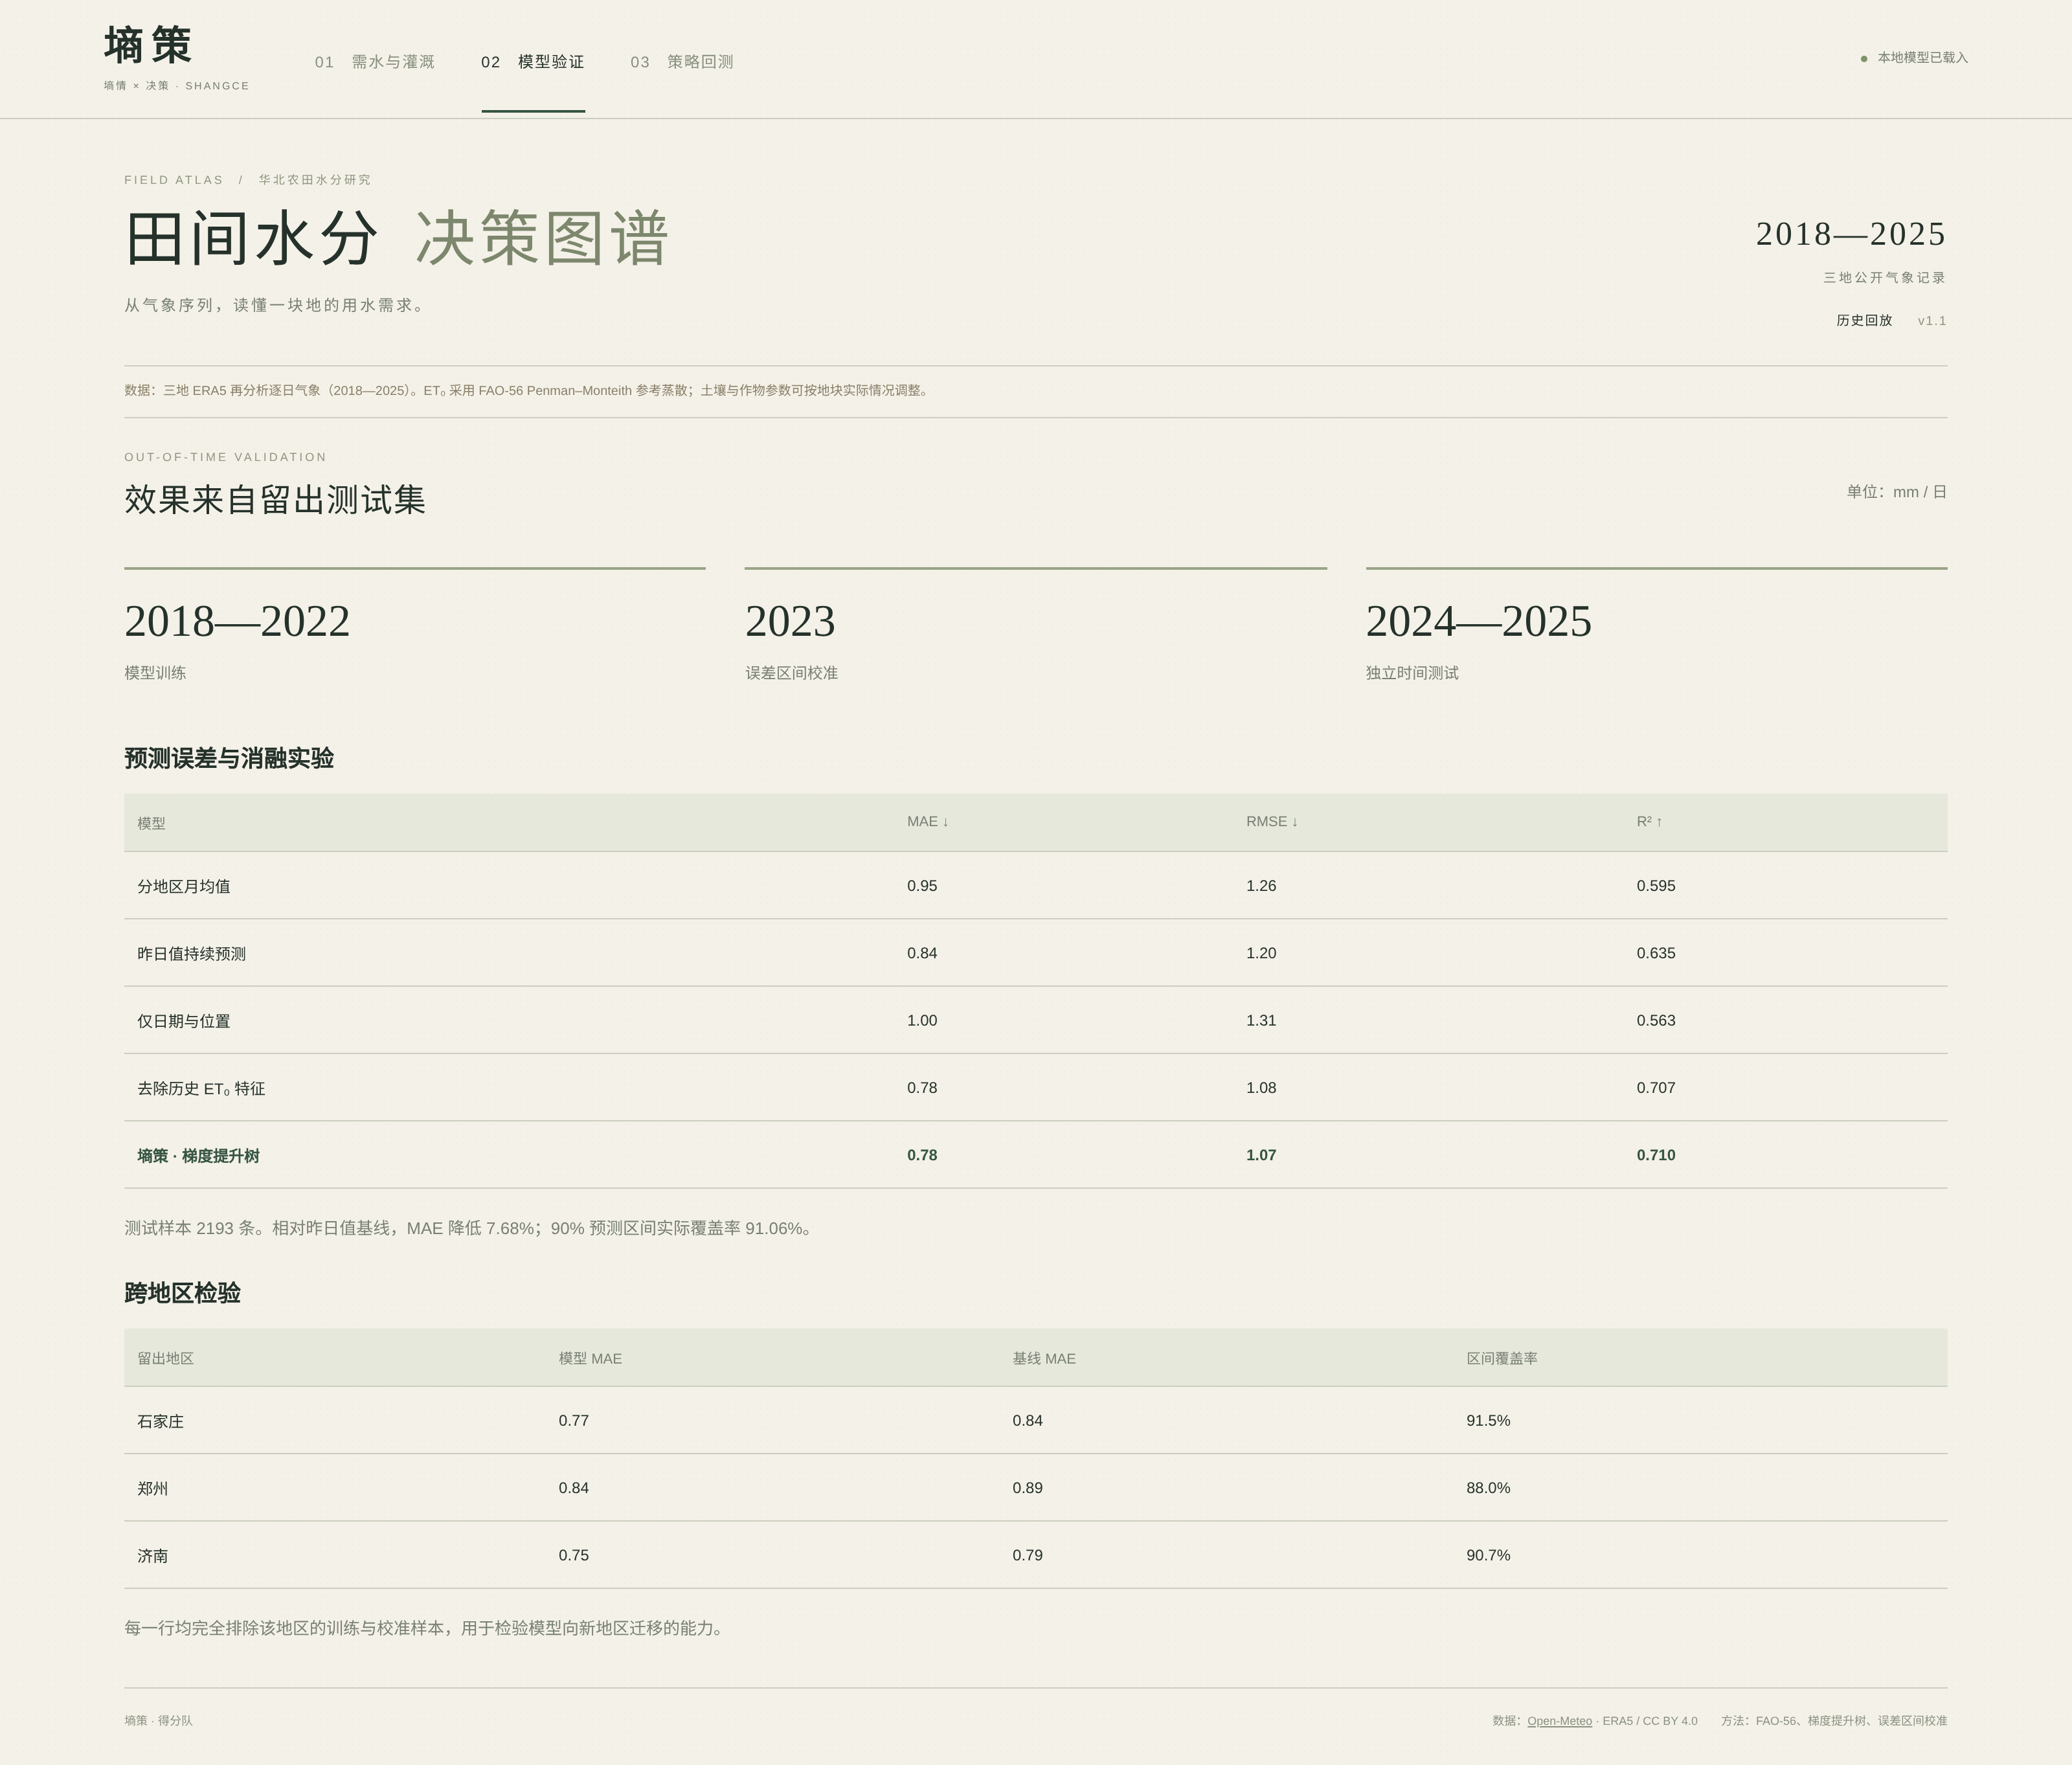
\includegraphics[width=.49\linewidth,height=.42\textheight,keepaspectratio]{../results/screenshots/evidence.png}\hfill
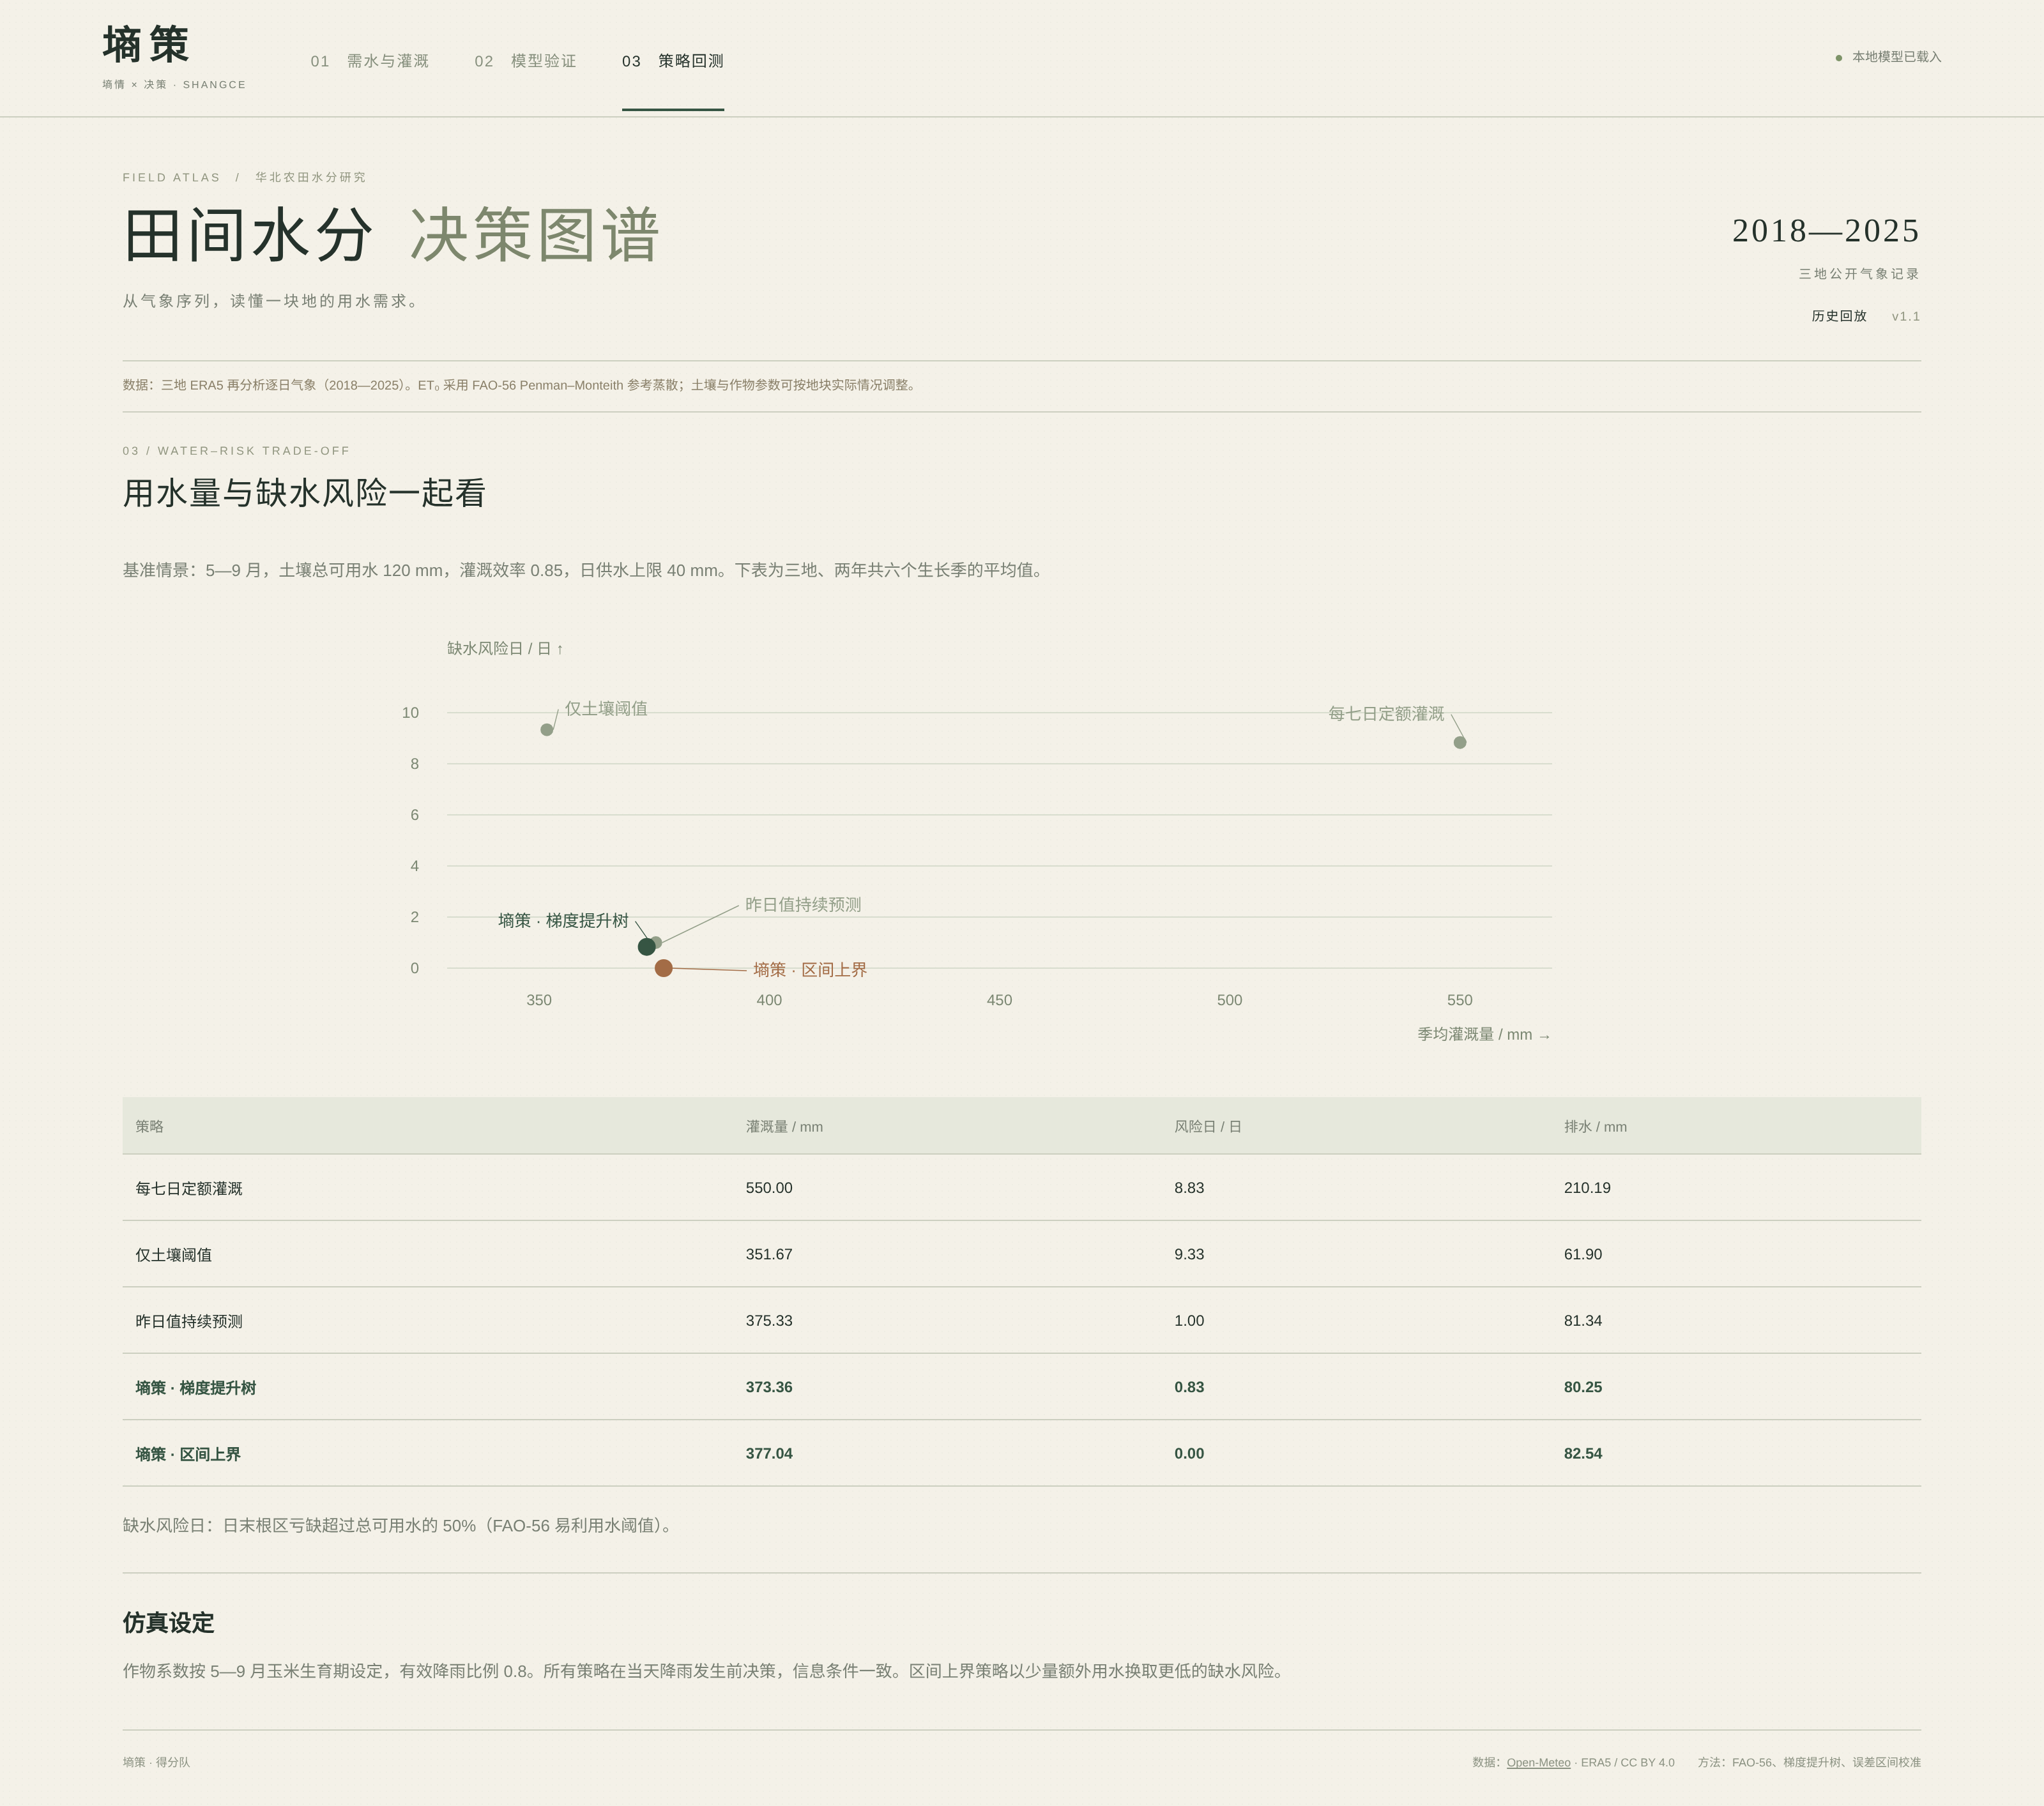
\includegraphics[width=.49\linewidth,height=.42\textheight,keepaspectratio]{../results/screenshots/simulation.png}
\caption{“模型验证”（左）与“策略回测”（右）视图}\label{fig:evidence-ui}
\end{figure}

\subsubsection{评价指标定义}
对标签$y_i$与预测$\widehat y_i$：
\begin{align}
\MAE&=\frac{1}{n}\sum_{i=1}^n|y_i-\widehat y_i|,\qquad
\RMSE=\sqrt{\frac{1}{n}\sum_{i=1}^n(y_i-\widehat y_i)^2},\\
R^2&=1-\frac{\sum_i(y_i-\widehat y_i)^2}{\sum_i(y_i-\bar y)^2}.
\end{align}
区间评价采用经验覆盖率与平均宽度：
\begin{equation}
\widehat{\mathrm{Cov}}=\frac1n\sum_i\mathbf1(y_i\in[L_i,U_i]),\qquad
\bar\ell=\frac1n\sum_i(U_i-L_i).
\end{equation}
误差单位均为mm/日。覆盖率与宽度需要同时报告：区间过宽会使上界策略过度灌溉，过窄则在高需水期失去保护作用。

\subsection{预测精度}
\datatable{overall}{完整模型与对照方法的时间留出测试结果}{tab:overall}{三地2024—2025年共2193条样本，所有方法在测试期均未调参。}

如表\ref{tab:overall}所示，完整模型的MAE为0.7757 mm/日，在五种方法中最低，较昨日值基线（0.8403 mm/日）降低
\begin{equation}
100\%\times\left(1-\frac{0.775680}{0.840251}\right)=7.68\%,
\end{equation}
RMSE由1.1994降至1.0688 mm/日，$R^2$由0.6352提高到0.7103。仅用日期与位置的模型MAE为0.9951 mm/日，甚至不如地区月均值，说明完整模型的优势主要来自近期多变量气象信息，而非模型复杂度本身。

对两种方法逐日绝对误差之差，按日期平均三地后以14日为块做1000次块自助重采样，得到MAE差值的95\%区间为[0.0332, 0.0965] mm/日，区间不含0，表明完整模型相对昨日值的改进是稳定的，而非偶然波动。

\datafigure{residual.pdf}{测试期预测散点与残差分布（残差=预测−参考）}{fig:residual}

图\ref{fig:residual}显示预测值紧密分布在1:1线两侧。残差均值为$-0.087$ mm/日，整体略有低估；绝对误差中位数0.547 mm/日，90\%与95\%分位数分别为1.791和2.253 mm/日。完整模型在54.72\%的测试日误差小于昨日值。

\subsection{分地区与消融分析}
\datatable{site_year}{完整模型的地区—年份分组表现}{tab:siteyear}{该表模型训练时包含三地，属于分组评价。}

三地两年的六个分组中，模型MAE全部低于昨日值（表\ref{tab:siteyear}）。改进最明显的是郑州2024年（0.749对0.873，降低14.2\%）和济南2024年（降低9.5\%）；郑州2025年改进最小（0.896对0.905），且覆盖率为89.04\%，略低于名义水平，是后续优化需要关注的分组。

消融实验中，去除全部历史ET\textsubscript{0}特征后MAE仅由0.7757升至0.7800 mm/日。这说明历史气温、辐射、湿度、风速等原始变量已包含参考蒸散的大部分信息，模型并不依赖平台计算的历史ET\textsubscript{0}，这有利于今后改用地面气象站数据作为输入。

\subsection{预测区间的覆盖与季节诊断}
测试期名义90\%区间的整体经验覆盖率为91.06\%，平均宽度3.61 mm/日；2193条样本中102条落在下界以下、94条高于上界，两侧失覆盖数量接近，区间没有系统性偏向。

\datafigure{seasonality.pdf}{分月MAE与经验覆盖率（虚线为90\%名义水平，棕色柱表示低于名义水平）}{fig:seasonality}

\datatable{monthly}{测试集分月误差、偏差与覆盖率}{tab:monthly}{偏差为预测减参考；覆盖率按该月三地两年合并计算。}

进一步按月份分解（图\ref{fig:seasonality}、表\ref{tab:monthly}），模型误差呈明显季节性：1月MAE仅0.303 mm/日，6月升至1.268 mm/日。由于区间采用全年统一的半宽$q$，冬季区间偏宽、覆盖率达100\%，而6月和7月覆盖率降至78.33\%和79.03\%。值得注意的是，即便在夏季，模型MAE仍低于昨日值（6月1.268对1.456），点预测的优势没有消失，问题出在区间宽度没有随季节自适应。这一发现直接指向第\ref{sec:outlook}章的改进方案：按季节或按预测误差尺度分别校准。

\datafigure{coverage_heatmap.pdf}{地区—月份经验覆盖率（\%）}{fig:heatmap}

图\ref{fig:heatmap}按地区细分了同一现象，三地夏季覆盖率均有不同程度下降，说明这是方法层面的共性问题，而非某一地区的数据异常。

\subsection{极端误差样本分析}
\datatable{worst}{绝对误差最大的八条测试记录}{tab:worst}{单位mm/日，按绝对误差从大到小排序。}

表\ref{tab:worst}列出误差最大的八条样本，集中在6月前后。例如郑州2024年6月16日，前一日参考值高达7.28 mm/日，当日骤降至1.81 mm/日，模型预测6.54 mm/日，虽已较昨日值有所修正，仍明显偏高。图\ref{fig:failure}显示该时段伴随明显降水过程。

\datafigure{failure_case.pdf}{郑州2024年6月误差案例窗口（降水为事后实况，不参与预测）}{fig:failure}

这类误差源于“仅凭历史信息难以预知次日天气突变”。在实际部署中接入次日天气预报（降水概率、云量、气温预报）作为输入，是降低此类误差最直接的手段。

\subsection{跨地区迁移}
\datatable{transfer}{完全留出目标地区的迁移检验}{tab:transfer}{每次在其余两地训练与校准，目标地区不参与这两个阶段。}

在完全没见过目标地区数据的条件下，三地点预测MAE均低于该地昨日值基线，石家庄、郑州、济南分别降低8.4\%、5.3\%和5.5\%；石家庄与济南的区间覆盖率保持在90\%以上，郑州为87.96\%。这表明模型具备向相似气候区推广的潜力；部署到新地区时，可尝试用当地一年数据重新校准区间以提高覆盖可靠性，这一做法有待在新地区实测验证。

\subsection{灌溉策略仿真}
\datatable{central}{基准情景下五种策略的六季平均结果}{tab:central}{TAW=120 mm、$\eta=0.85$，其余参数见表\ref{tab:assumptions}。}

表\ref{tab:central}给出基准情景下的结果。与定额日历相比，三种预测型策略的季均用水减少约31\%\,$\sim$\,32\%，风险日从8.83日降至1日及以下。与只看当前墒情的阈值策略相比，预测型策略多用约22\,$\sim$\,25 mm水，但仿真风险日从9.33日降至0\,$\sim$\,1日，说明“提前看一天”可以明显减少模型中的缺水风险日。AI区间上界策略在基准情景六个生长季中均未出现风险日，季均用水377.04 mm，仅比AI点预测多3.7 mm。

\datafigure{season_trace.pdf}{郑州2024年基准情景下的日末亏缺与累计灌溉（上图虚线为60 mm触发线）}{fig:trace}

逐日轨迹（图\ref{fig:trace}）显示，墒情阈值策略要等亏缺越过触发线后才补水，在高需水日多次短暂越线；预测型策略在越线前一天提前补水，其中上界策略的亏缺曲线全季位于触发线下方。累计用水曲线呈阶梯状，三种策略的季节总量相差不大，差别主要体现在补水时机上。

\datatable{six_seasons}{基准情景中点预测与上界策略的逐季结果}{tab:seasons}{用水为单季毛灌溉量（mm），风险为单季风险日数。}

\datafigure{tradeoff_all.pdf}{全部180组仿真的用水量—风险日分布（每种策略36个环境情景）}{fig:alltradeoff}

\datatable{paired}{AI区间上界策略相对各参照策略的环境内配对比较}{tab:paired}{差值为上界策略减参照，最后一列为36个情景中风险日减少/相同/增加的次数。}

为排除土壤与效率差异的干扰，表\ref{tab:paired}在每个环境情景内配对比较。相对于AI点预测，上界策略平均多用5.65 mm水，平均减少1.25个风险日，36个情景中27个风险更低、9个持平、0个更高；相对于墒情阈值策略，36个情景全部降低风险，平均减少11.25个风险日。上界策略为使用者提供了一个明确的“以少量用水换取更低风险”的选项。

\subsection{敏感性分析}
\datafigure{soil_sensitivity.pdf}{效率0.85时不同TAW下的六季平均用水与风险日}{fig:sensitivity}

图\ref{fig:sensitivity}和附录表\ref{tab:allsensitivity}显示：土壤储水越小（TAW=80 mm），各策略风险越高，不确定性信息的价值越突出——此时上界策略仍保持0风险日，而点预测为2.00日。灌溉效率由0.85降为0.70时，补足同样亏缺所需毛水量上升，40 mm日上限更容易成为约束。在全部6种“容量—效率”组合中，上界策略的风险日始终是五种策略中最低的（0\,$\sim$\,0.17日）；而AI点预测仅在基准组合中风险日低于昨日值，在其余5种组合中略高（差值0.17\,$\sim$\,0.67日）。这说明点预测精度的小幅提升不一定转化为更低的缺水风险，把误差区间纳入决策才是稳定降低风险的关键，这也印证了本作品“把预测误差放进灌溉决策”的设计思路。

\subsection{效益分析}
\textbf{节水与稳产潜力。}在6种“容量—效率”组合下（各为三地两年平均），AI区间上界策略相对于定额日历灌溉节约用水11\%\,$\sim$\,37\%（基准情景31.4\%），同时风险日不超过0.17日；相对于仅凭墒情阈值灌溉，以小幅增加用水换取缺水胁迫的大幅减少。这些结果来自统一参数下的仿真，实际节水与产量效益将通过田间影子运行和对照试验进一步验证（第\ref{sec:outlook}章）。

\textbf{社会效益。}系统完全离线运行、单次推理约11.5 ms、模型仅416 KiB，对硬件和网络没有要求，适合在基层农技站、合作社推广；界面直观展示“为什么要灌、为什么灌这么多”，有助于把科学灌溉方法传递给农户。

\textbf{教学与科研效益。}系统可作为农业水利、智慧农业课程的教学工具，学生能在同一天气条件下改变土壤、作物与设备参数，直观理解FAO-56水量平衡；完整开放的数据、代码与逐日结果也便于他人复现与扩展研究。
